%! TEX root = ../tor.tex

\chapter{Design}

\indent\indent Rețeaua Tor este una care se adaugă peste rețeaua existentă (eng.\ %
\texttt{overlay network}). \index{overlay network} Fiecare OR funcționează
ca un proces inițiat de utilizator, fără privilegii speciale. OR păstrează
o conexiune TLS cu toate celelalte OR, iar utilizatorii rulează
software local, numit \emph{onion proxy} (OP) \index{onion!proxy (OP)} pentru
a obține directoarele, a stabili circuite în rețea și a administra
conexiuni cu aplicații ale utilizatorului. Aceste OP acceptă fluxuri TCP
și le trimit în format multiplex prin circuit. OR din capătul celălalt
conectează destinațiile cerute și pune datele la dispoziție.

Fiecare OR ține o \textit{cheie de identitate} pe termen lung și o \textit{cheie onion}
pe termen scurt. \index{cheie!de identitate} \index{cheie!onion}
Cheia de identitate este folosită pentru semnarea
certificatelor TLS, pentru semnarea descriptorului OR (care conține un
rezumat al cheilor, adreselor, lățimii de bandă, politicilor de ieșire etc.) și,
prin serverele directoare, să semneze directoarele.

Cheie onion este folosită pentru a decripta cererile utilizatorilor, a stabili
circuitele și a negocia cheile efemere.

Protocolul TLS stabilește o cheie de legătură pe termen scurt
atunci cînd comunică între OR. Toate cheile de termen scurt sînt rotite periodic
și independent.

%%%%%%%%%%%%%%%%%%%%%%%%%%%%%%%%%%%%%%%%%%%%%%%%%%%%%%%%%%%%%%%%%%%%%%
\section{Celule}

\indent\indent OR comunică între ele și cu utilizatorii prin conexiuni TLS cu chei efemere.
Astfel se ascund datele conexiunii cu securitate perfectă la înaintare
(eng.\ \texttt{perfect forward secrecy}), împiedicînd orice atacator să
modifice date pe drum sau să pretindă că este un OR.
\index{securitate!perfectă la înaintare}

Traficul între OR circulă în \emph{celule}, fiecare avînd mărimea de 512 octeți.
Celulele sînt alcătuite dintr-un cap (\emph{header}) și o încărcătură
(\emph{payload}). \index{celule}
\index{celule!cap (header)}
\index{celule!încărcătură (payload)}

Capul conține un identificator al circuitului prin care trece celula respectivă
(dat fiind că mai multe fire TLS sînt trecute prin același circuit, în format
multiplex) și o comandă care specifică ce să se întîmple cu sarcina
din celulă. Indetificatorul circuitului este unic pentru fiecare conexiune.

Pe baza comenzilor, celulele pot fi \emph{de control}, care sînt mereu
interpretate de nodul care le primește, sau \emph{de transfer}, care
cară informație. \index{celule!de control} \index{celule!de transfer}
\index{celule!comenzi}
Comenzile din celulele de control sînt:
\begin{itemize}
  \item \texttt{padding}, folosită pentru \texttt{TCP keepalive}\footnote{\url{http://tldp.org/HOWTO/TCP-Keepalive-HOWTO/overview.html}}, dar și pentru securitate, cf.\ \S\ref{sec:idei}.
  \item \texttt{create} sau \texttt{created}, pentru organizarea unui
    nou circuit, respectiv confirmarea reușitei;
  \item \texttt{destroy}, pentru eliminarea circuitului curent.
\end{itemize}

Celulele de transfer (eng.\ \texttt{relay}) au un cap suplimentar, care
specifică fluxul de date pentru celula respectivă, apoi o sumă de
control bidirecțională (eng.\ \texttt{end to end check\-sum}) pentru a
asigura integritatea, lungimea sarcinii ce se va transfera și comanda
de transfer. Conținutul capului și sarcinii din celula de transfer
sînt criptate cu cifrul AES pe 128 biți.

Comenzile de transfer sînt:
\begin{itemize}
  \item \texttt{relay data}, pentru datele care circulă pe acel fir;
  \item \texttt{relay begin}, pentru începutul transferului;
  \item \texttt{relay teardown}, pentru a închide un transfer stricat;
  \item \texttt{relay connected}, pentru a notifica reușita conexiunii;
  \item \texttt{relay extend} și \texttt{relay extended}, pentru a mai
    face un pas în conexiune și a notifica de el;
  \item \texttt{relay truncate} și \texttt{relay truncated}, pentru distrugerea
    unei părți de circuit și notificare;
  \item \texttt{relay sendme} pentru rezolvarea congestiilor;
  \item \texttt{relay drop} pentru implementarea long range dummies.\footnote{celule %
      \qq{zgomot} care pot fi distinse de datele normale abia
    la ultimul pas, cf.\ \href{https://lists.torproject.org/pipermail/tor-dev/2002-July/001127.html}{M.\ Pfajfar}.}
\end{itemize}

%%%%%%%%%%%%%%%%%%%%%%%%%%%%%%%%%%%%%%%%%%%%%%%%%%%%%%%%%%%%%%%%%%%%%%

\section{Construcția unui circuit}

\indent\indent OP-ul unui utilizator construiește un circuit din aproape
în aproape, negociind cîte o cheie simetrică cu fiecare OR de pe drum.

Fie Alice utilizatorul care lansează cererea. El trimite o celulă cu
comanda \texttt{create} către primul nod din drumul ales, fie el Bob.
Alice alege un \texttt{circID} $C_{AB}$ pentru această conexiune.
Sarcina primei celule create conține prima jumătate a criptării
\emph{Diffie-Hellman handshake} ($g^x$), criptată ca fiind cheia onion
a OR-ului. Bob răspunde cu celula care conține comanda \texttt{created},
care conține $ g^y $ și un hash al cheii complet negociate, $ K = g^{xy} $.
\index{criptare!Diffie-Hellman}

\vspace{1cm}
Facem o mică digresiune pentru a aminti funcționarea criptării Diffie-Hellman.
Detalii și alte explicații preluate de la \cite{dhse}.
Pașii sînt următorii:
\begin{enumerate}[(1)]
  \item Alice alege două numere prime $ g $ și $ p $ și le transmite lui Bob.
  \item Bob alege un număr secret $ a $, pe care nu-l transmite nimănui.
    El calculează apoi $ A = g^a \text{ mod } p $ și transmite rezultatul lui Alice.
  \item Alice alege un număr secret $ b $ și face un calcul similar,
    adică $ B = g^b \text{ mod } p $ și transmite lui Bob rezultatul.
  \item Bob calculează acum $ B^a \text{ mod } p $, iar Alice calculează
    $ A^b \text{ mod } p $, iar amîndoi obțin a\-ce\-lași rezultat.
    Aceasta deoarece au loc egalitățile:
    \begin{align*}
      (g^a \text{ mod } p)^b \text{ mod } p &= g^{ab} \text{ mod p} \\
      (g^b \text{ mod } p)^a \text{ mod } p &= g^{ba} \text{ mod p}
    \end{align*}
\end{enumerate}
\vspace{1cm}

După stabilirea circuitului, Alice și Bob își pot trimite mesaje folosind
cheia $ K $.

Pentru extinderea ulterioară a circuitului, Alice trimite o celulă cu
comanda \texttt{relay extend} către Bob, în care specifică adresa
următorului OR pe care vrea să-l acceseze, să zicem Carol, și partea
$ g^{x_2} $ a cheii pentru el. Bob își face o copie a jumătății de cheie
$ g^{x_2} $ și trimite o celulă \texttt{create} către Carol. Totodată,
Bob își alege un \texttt{circID} pentru legătura cu Carol, pe care Alice
poate să nu-l știe; este suficient ca Bob să lege $ C_{AB} $ de $ C_{BC} $.

Carol răspunde cu o celulă \texttt{created} către Bob și cheia $ g^{y_2} $, 
iar Bob apoi trimite sarcina către Carol și răspunde cu \texttt{relay extended} către Alice.
Acum circuitul este extins și legătura A--C se poate face cu cheia
$ K_2 = g^{x_2y_2} $.

Procesul continuă analog pentru extinderi ulterioare.

Protocolul unilateral de handshake la nivel de circuit permite ca Alice să
știe cu ce OR face legătura, dar OR-ul să nu știe --- astfel se
păstrează anonimitatea celulei care lansează cererea. Nu există chei publice
în această legătură, iar autentificarea este unilaterală (Alice și OR
negociază cheia, iar Alice știe doar că OR a învățat cheia din cele
două jumătăți).

Protocolul are, totodată, secret la înaintare și noutate a cheilor.

Formal, fie $ E_{PK_{Bob}} $ criptarea cu cheia lui Bob, $ H $ este funcția
hash, iar $ \mid $ este concatenarea. Avem:
\begin{itemize}
  \item Alice $ \longrightarrow $ Bob: $E_{PK_{Bob}}(g^x) $;
  \item Bob $ \longrightarrow $ Alice: $ g^y, H$ ($ K \mid$ ``handshake'').
\end{itemize}

În a doua parte, Bob arată că el este cel care primește $ g^x $ și alege
$ y $-ul corespunzător. În primul pas se folosește cheie publică, deoarece
celula este prea mică pentru a stoca o cheie publică și semnătura.

Schema acestei conexiuni, cu tot cu celule și chei este redată în figura \ref{fig:cells}.

\begin{figure}[!htbp]
  \centering
  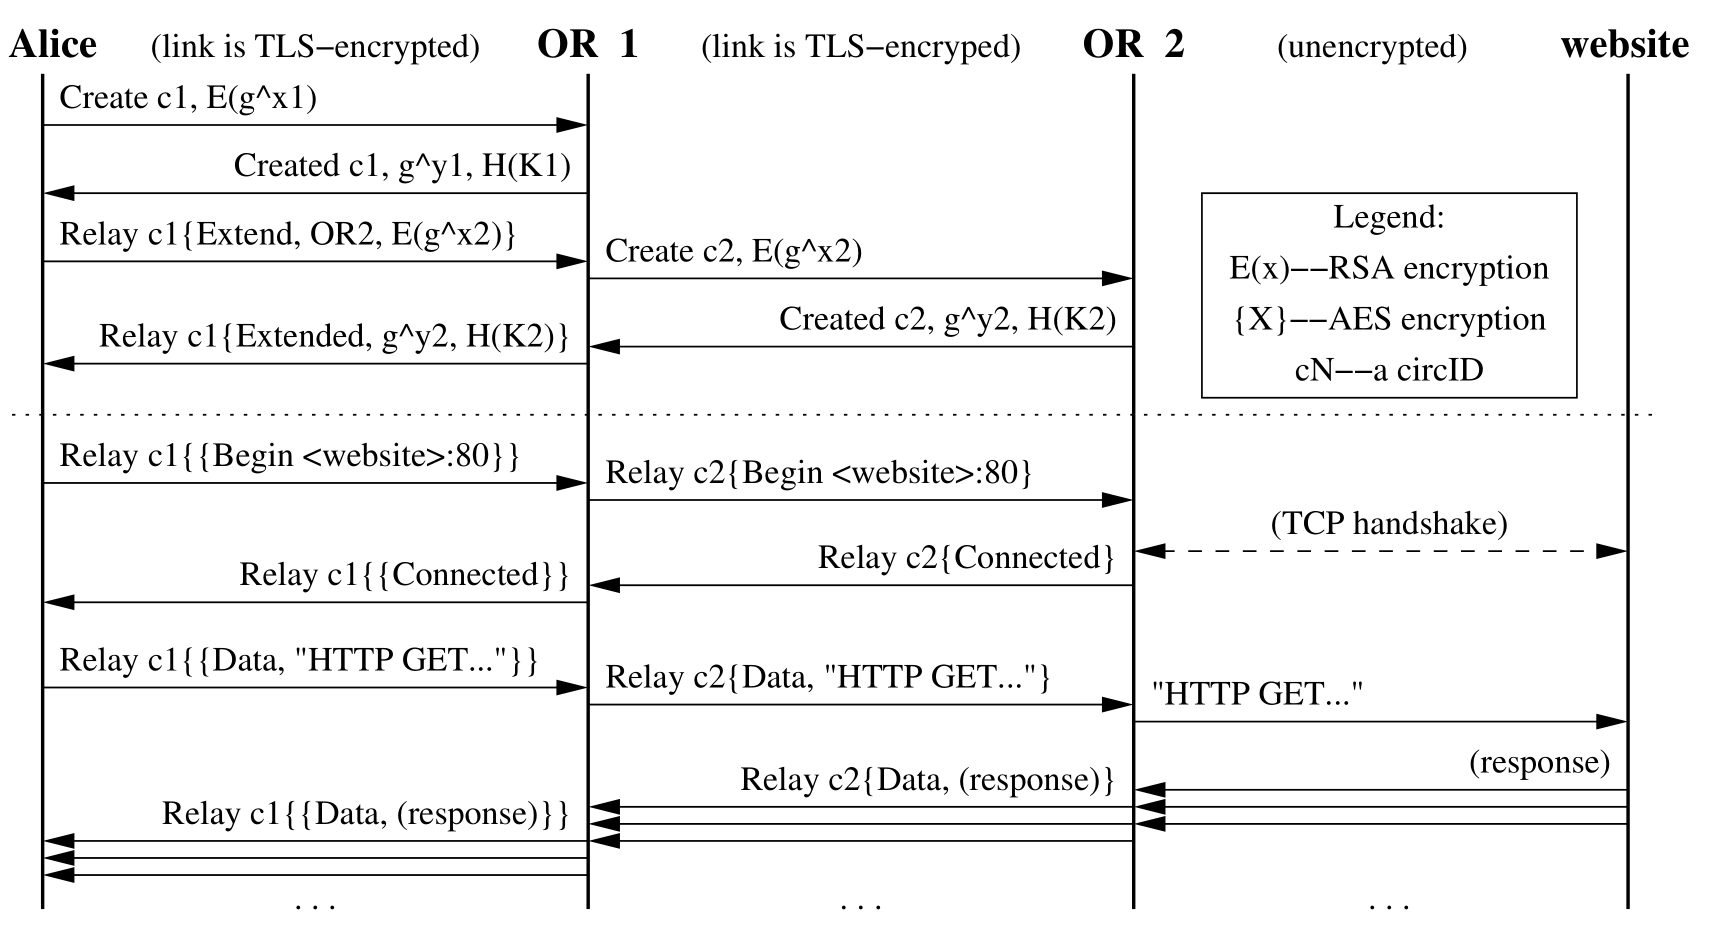
\includegraphics{fig/cells.png}
  \caption{Celulele schimbate la inițierea unui circuit, cf.\ \cite{whitepaper}, \S4.1}
  \label{fig:cells}
\end{figure}



\vspace{1cm}

Alte detalii despre protocolul Tor și specificațiile oficiale se pot
găsi pe \href{https://gitweb.torproject.org/torspec.git/tree/}{site-ul oficial}.
